% Coherence Collapse Analysis: The Chronometry of Coherence in Networked Systems
% A formal method for failure mode identification in sociotechnical systems

\documentclass[11pt,a4paper]{article}

% Core packages
\usepackage[utf8]{inputenc}
\usepackage[T1]{fontenc}
\usepackage{amsmath,amssymb,amsthm}
\usepackage{mathtools}
\usepackage{graphicx}
\usepackage{xcolor}
\usepackage{hyperref}
\usepackage{cleveref}
\usepackage{booktabs}
\usepackage{array}
\usepackage{float}
\usepackage{enumitem}
\usepackage{tikz}
\usetikzlibrary{shapes,arrows,positioning,calc}
% Algorithm formatting removed - using enumitem instead
\usepackage[margin=1in]{geometry}

% Theorem environments
\theoremstyle{definition}
\newtheorem{definition}{Definition}[section]
\newtheorem{theorem}{Theorem}[section]
\newtheorem{lemma}[theorem]{Lemma}
\newtheorem{corollary}[theorem]{Corollary}
\newtheorem{proposition}[theorem]{Proposition}
\newtheorem{axiom}{Axiom}

\theoremstyle{remark}
\newtheorem{remark}{Remark}[section]
\newtheorem{example}{Example}[section]

% Custom commands
\newcommand{\keff}{k_{\text{eff}}}
\newcommand{\Kreq}{K_{\text{req}}}
\newcommand{\Ttruth}{T_{\text{truth}}}
\newcommand{\Tentropy}{T_{\text{entropy}}}
\newcommand{\Tcapture}{T_{\text{capture}}}
\newcommand{\Teff}{T_{\text{eff}}}
\newcommand{\rhocrit}{\rho_{\text{crit}}}
\newcommand{\sigmin}{\sigma_{\text{min}}}
\newcommand{\R}{\mathbb{R}}
\newcommand{\N}{\mathbb{N}}
\newcommand{\E}{\mathbb{E}}
\newcommand{\Prob}{\mathbb{P}}

% Colors for diagrams
\definecolor{chaosblue}{RGB}{52,152,219}
\definecolor{healthygreen}{RGB}{46,204,113}
\definecolor{rigidityred}{RGB}{231,76,60}
\definecolor{singularitypurple}{RGB}{155,89,182}

% Hyperref setup
\hypersetup{
    colorlinks=true,
    linkcolor=blue!60!black,
    citecolor=green!50!black,
    urlcolor=blue!70!black
}

\title{\textbf{Coherence Collapse Analysis}\\[0.5em]
\large A Universal Failure Mode in Complex Coordinating Systems}

\author{
Eric Moore\\
\texttt{eric@ciris.ai}
}

\date{January 2026}

\begin{document}

\maketitle

\begin{abstract}
\textbf{We present evidence for a cross-domain failure mode in complex coordinating systems: correlation-driven diversity collapse.} As constraints governing system behavior become correlated, effective diversity collapses toward unity regardless of nominal scale---a phenomenon we formalize as $\keff = k/(1+\rho(k-1)) \to 1$ as $\rho \to 1$. This collapse is thermodynamically favored, invisible until catastrophic, and---critically---\textbf{tested across three independent scientific domains}: lithium-ion battery degradation (NASA dataset, 19 cells), institutional failure (Quality of Government + Polity V, 203 countries), and microbiome dysbiosis (American Gut Project, 2,081 taxa). The $\keff$ formula provides consistent structural mappings across all domains. Phase classification (chaos/healthy/rigidity) is reliable; timing estimates carry higher uncertainty.

We derive three collapse timelines ($\Ttruth$, $\Tentropy$, $\Tcapture$) with closed-form expressions, identify a singularity boundary ($\Kreq \cdot \rho \geq 1$) beyond which recovery becomes impossible, and establish information-theoretic limits on detection. The framework---\textbf{Coherence Collapse Analysis (CCA)}---is validated through Monte Carlo simulation and formal verification in Lean 4.

\textbf{Implications}: If these findings generalize, correlation accumulation represents a candidate mechanism for systemic failure at civilizational scale. AI systems are significant not because they are uniquely dangerous, but because they accelerate correlation ($\rho \uparrow$) faster than any prior technology while appearing to increase constraint count ($k \uparrow$)---masking diversity collapse until the system crosses irreversible thresholds.

\medskip
\noindent\textbf{Scope:} \textit{CCA is an \textbf{engineering risk framework} for identifying structural failure modes and intervention windows. The cross-domain validation demonstrates generality. Its value lies in making hidden fragility legible before collapse becomes irreversible.}
\end{abstract}

\tableofcontents
\newpage

%==============================================================================
\section{Introduction: The Hypothesis}
%==============================================================================

\subsection{The Core Claim}

We propose that complex coordinating systems---whether biological, chemical, institutional, or artificial---share a common failure mode:

\begin{quote}
\textbf{Correlation accumulation drives effective diversity toward unity, rendering systems fragile to perturbation regardless of nominal scale.}
\end{quote}

This claim is formalized through the \textit{effective constraint count}:
\begin{equation}
\keff = \frac{k}{1 + \rho(k-1)}
\end{equation}
where $k$ is the number of constraints (rules, precedents, species, cells) and $\rho$ is their average pairwise correlation. As $\rho \to 1$, $\keff \to 1$ regardless of $k$. A system with 1,000 highly correlated constraints has the effective diversity of a system with one.

\subsection{The Evidence}

This claim would be speculative without cross-domain validation. We tested the $\keff$ formula and associated collapse dynamics against three authoritative empirical datasets from unrelated scientific domains:

\begin{table}[H]
\centering
\begin{tabular}{llll}
\toprule
\textbf{Domain} & \textbf{Dataset} & \textbf{Structural Accuracy} & \textbf{Timing Uncertainty} \\
\midrule
Chemistry & NASA Li-ion (19 cells) & 8.1\% RMSE & Overestimates final SOH by $\sim$8\% \\
Political Science & QoG + Polity V (203 countries) & 5/5 true negatives & 3/13 false positives; 7.6yr early \\
Biology & American Gut (2,081 taxa) & Matches AGP norms & FMT dynamics simplified \\
\bottomrule
\end{tabular}
\caption{Cross-domain validation summary. Note: The $\keff$ formula is an \textit{identity}---it computes effective constraints from measured $k$ and $\rho$. Validation tests whether this mapping produces useful structural analysis.}
\end{table}

The same mathematics describes battery cell degradation, institutional collapse, and microbiome dysbiosis. This generality suggests we have identified a \textit{structural property of constraint-based systems}, not a domain-specific artifact. However, three domains do not establish universality---they demonstrate cross-domain applicability that warrants further testing.

\subsection{The Implications}

If this failure mode is universal, it has consequences beyond any single domain:

\begin{enumerate}[noitemsep]
    \item \textbf{The failure is invisible}: Systems accumulate correlation while appearing healthy ($k$ grows). The collapse of $\keff$ is not directly observable without measuring $\rho$.

    \item \textbf{The failure is thermodynamically favored}: Correlation is lower-entropy than diversity. Without active maintenance, systems drift toward homogeneity.

    \item \textbf{AI accelerates the failure asymmetrically}: AI systems increase constraint count ($k \uparrow$) and correlation ($\rho \uparrow \uparrow$) simultaneously, while externalizing sustainability costs ($\sigma \downarrow$). This masks diversity collapse behind apparent scale.
\end{enumerate}

This positions correlation accumulation as a \textit{candidate Great Filter}---not because AI is uniquely dangerous, but because technological coordination accelerates correlation faster than systems can renew diversity.

\subsection{The Framework}

\textbf{Coherence Collapse Analysis (CCA)} is the formal apparatus for analyzing this failure mode. It synthesizes techniques from:
\begin{itemize}[noitemsep]
    \item Failure Mode and Effects Analysis (FMEA) in safety engineering
    \item Stability analysis in control theory
    \item Phase transition analysis in statistical mechanics
    \item Information-theoretic bounds from detection theory
\end{itemize}

CCA provides:
\begin{enumerate}[noitemsep]
    \item \textbf{Failure modes}: How coherence is lost (deception, entropy, capture)
    \item \textbf{Attractor states}: Where systems tend to drift (chaos vs. rigidity)
    \item \textbf{Intervention windows}: When corrective action remains effective
    \item \textbf{Detection limits}: What can and cannot be observed
\end{enumerate}

\subsection{Scope and Falsifiability}

\begin{table}[H]
\centering
\begin{tabular}{>{\raggedright}p{0.45\textwidth} >{\raggedright\arraybackslash}p{0.45\textwidth}}
\toprule
\textbf{CCA Is} & \textbf{CCA Is Not} \\
\midrule
Structural analysis of failure conditions & Prediction of historical outcomes \\
Identification of phase boundaries & Fortune-telling or prophecy \\
Cross-domain validated mathematics & Universal law (yet) \\
Engineering-style failure analysis & Social physics or psychohistory \\
Falsifiable framework & Unfalsifiable speculation \\
\bottomrule
\end{tabular}
\caption{Scope boundaries for Coherence Collapse Analysis}
\end{table}

The framework is falsified if:
\begin{itemize}[noitemsep]
    \item The $\keff$ formula fails in additional domains
    \item Systems with high $\rho$ demonstrate sustained resilience
    \item Correlation accumulation reverses spontaneously without intervention
\end{itemize}

\subsection{Contributions}

This paper makes the following contributions:
\begin{enumerate}
    \item \textbf{Cross-domain validation} of the $\keff$ framework against NASA battery data, QoG/Polity institutional data, and American Gut Project microbiome data (consistent structural mappings; reliable phase classification).

    \item A formal definition of the \textbf{defense function} $J$ that unifies scale, diversity, integrity, and sustainability into a single quantity. (Note: $J$ is a \textit{modeling choice}, not a derived result---its value lies in whether it produces useful analysis, not in theoretical necessity.)

    \item Derivation of \textbf{three collapse timelines} ($\Ttruth$, $\Tentropy$, $\Tcapture$) with closed-form expressions and identified singularities.

    \item Characterization of the \textbf{chaos-rigidity phase space} and the narrow corridor of sustainable coherence.

    \item Information-theoretic proof that \textbf{a non-trivial class of emergent incoherence is fundamentally undetectable} (the L-01 barrier).

    \item A \textbf{stability condition} ($\alpha/\keff > d$) that distinguishes growing from decaying systems.

    \item Formal verification of key theorems in \textbf{Lean 4} with Mathlib dependencies.

    \item An \textbf{open-source implementation} with Python modules, Lean proofs, and simulation scripts (\texttt{github.com/CIRISAI/RATCHET}).
\end{enumerate}

%==============================================================================
\section{Mathematical Foundations}
%==============================================================================

\subsection{Constraint Geometry}

The foundation of CCA is the observation that system coherence is maintained through \textit{constraints}---rules, precedents, norms, or structural features that limit the space of possible behaviors.

\begin{definition}[Constraint Space]
A \textbf{constraint space} is a tuple $(V, \mathcal{C}, \rho)$ where:
\begin{itemize}[noitemsep]
    \item $V \subseteq \R^n$ is the space of possible system states
    \item $\mathcal{C} = \{C_1, \ldots, C_k\}$ is a set of constraint halfspaces
    \item $\rho: \mathcal{C} \times \mathcal{C} \to [0,1]$ is the pairwise correlation function
\end{itemize}
\end{definition}

The \textit{feasible region} is the intersection $\bigcap_{i=1}^{k} C_i$, representing states consistent with all constraints. Deceptive or incoherent behaviors correspond to states outside this region.

\begin{definition}[Effective Constraint Count]
Given $k$ constraints with average pairwise correlation $\rho$, the \textbf{effective constraint count} is:
\begin{equation}
\keff = \frac{k}{1 + \rho(k-1)}
\label{eq:keff}
\end{equation}
\end{definition}

\begin{remark}[Statistical Provenance]
This formula is mathematically identical to the \textbf{Kish design effect} for effective sample size in survey statistics, which accounts for autocorrelation in clustered samples. We do not claim novelty for the formula itself---only for its application to constraint-based system analysis. The ``validation'' of $\keff$ across domains confirms that the algebra of effective sample sizes holds when variables are appropriately mapped; it does not establish that such mappings are causally meaningful in all contexts.
\end{remark}

This captures the intuition that correlated constraints provide redundant information:
\begin{itemize}[noitemsep]
    \item When $\rho = 0$ (independent): $\keff = k$
    \item When $\rho \to 1$ (fully correlated): $\keff \to 1$
\end{itemize}

\begin{theorem}[Volume Decay]
Under the following assumptions:
\begin{enumerate}[noitemsep,label=(\alph*)]
    \item Constraints are drawn i.i.d.\ from a distribution over halfspaces with bounded support
    \item The initial feasible region $V_0$ is bounded and convex
    \item Constraint normals have mean zero and covariance $\Sigma$ with $\|\Sigma\| \leq M$ for some $M > 0$
\end{enumerate}
the volume of the feasible region decays exponentially with effective constraints:
\begin{equation}
V(k) = V_0 \cdot e^{-\lambda \cdot \keff} \cdot (1 + O(1/\sqrt{\keff}))
\label{eq:volume_decay}
\end{equation}
where $\lambda > 0$ is the decay constant determined by constraint geometry, and the error term vanishes as $\keff \to \infty$.
\end{theorem}

\begin{proof}[Proof sketch]
Under assumption (a), each independent constraint removes a fraction of the remaining volume. By Gr\"unbaum's theorem on log-concavity of volume under halfspace intersection, the reduction is multiplicative. For $\keff$ effective (non-redundant) constraints, this yields $V(\keff) \approx V_0 \cdot \prod_{i=1}^{\keff} (1 - \delta_i)$ where $\delta_i$ is the fraction removed by constraint $i$. Taking logs and applying the law of large numbers under assumption (c), $\sum \ln(1-\delta_i) \approx -\lambda \cdot \keff$ for some $\lambda$ depending on the constraint distribution. The correlation adjustment ($\keff$ vs $k$) follows from the effective sample size formula: correlated constraints provide redundant information, reducing the effective count by factor $(1 + \rho(k-1))^{-1}$.
\end{proof}

\begin{remark}[Applicability]
The exponential form is an approximation valid when constraints are ``generic'' (no degenerate intersections) and sufficiently numerous. For small $k$ or highly structured constraint sets, empirical validation is required.
\end{remark}

\subsection{The Defense Function}

\begin{definition}[Defense Function]
The \textbf{defense function} $J$ quantifies the computational cost an adversary must pay to maintain incoherent behavior:
\begin{equation}
J = \keff \cdot (1 - \rho) \cdot \lambda \cdot \sigma
\label{eq:defense}
\end{equation}
where:
\begin{itemize}[noitemsep]
    \item $\keff$: Scale (effective constraints)
    \item $(1-\rho)$: Diversity (constraint independence)
    \item $\lambda$: Strictness (constraint strength)
    \item $\sigma$: Sustainability (maintenance capacity)
\end{itemize}
\end{definition}

\begin{remark}[Definitional Status of $J$]
The defense function $J$ is a \textbf{modeling choice}, not a derived quantity. We do not claim that $J$ is the unique or correct measure of system resilience---only that this particular combination of terms produces useful analysis across multiple domains. Alternative formulations (e.g., weighted products, nonlinear combinations) may be appropriate for specific applications.
\end{remark}

This formulation exhibits a conceptual duality: systems with high defense $J$ against incoherence also tend to have high capacity for coordinated flourishing. High-defense systems are also high-capacity systems.

\begin{proposition}[J-C Duality Interpretation]
Let $C$ denote an abstract ``capacity for coordinated flourishing.'' If we operationalize $C$ as the product of:
\begin{itemize}[noitemsep]
    \item effective coordination channels ($\keff$),
    \item independence of those channels ($1-\rho$),
    \item enforcement strength ($\lambda$), and
    \item resource sustainability ($\sigma$),
\end{itemize}
then $J = C$ by definition. This is not a derived result but a \textbf{definitional choice} that interprets defense and capacity as dual aspects of the same underlying quantity.
\end{proposition}

\begin{remark}
The J-C duality is interpretive rather than mathematical. It asserts that the same structural features that make a system hard to subvert also make it capable of positive coordination. This claim is falsifiable: if empirical systems show high $J$ with low flourishing capacity (or vice versa), the interpretation fails.
\end{remark}

The defense function provides a single scalar that summarizes system health. Its dynamics determine whether the system is growing stronger or collapsing.

\subsection{Stability Condition}

\begin{definition}[Collapse Rate]
The \textbf{collapse rate} is the time derivative of the defense function:
\begin{equation}
R_c = \frac{dJ}{dt}
\end{equation}
\end{definition}

\begin{theorem}[Stability Condition]
A system is stable if and only if $R_c \geq 0$. Under the simplifying assumption that $\lambda$ is constant, this reduces to:
\begin{equation}
\text{Stable} \iff \frac{\alpha}{\keff} > d
\label{eq:stability}
\end{equation}
where $\alpha = dk/dt$ is the constraint generation rate and $d$ is the sustainability decay rate.
\end{theorem}

\begin{proof}[Derivation]
From $J = \keff \cdot (1-\rho) \cdot \lambda \cdot \sigma$, apply the product rule:
\begin{equation}
\frac{dJ}{dt} = \lambda \left[ \frac{d\keff}{dt}(1-\rho)\sigma + \keff\left(-\frac{d\rho}{dt}\right)\sigma + \keff(1-\rho)\frac{d\sigma}{dt} \right]
\end{equation}

Assume the dominant dynamics are:
\begin{enumerate}[noitemsep,label=(\roman*)]
    \item $\keff$ grows proportionally to new constraints: $d\keff/dt \approx \alpha / (1 + \rho(k-1))$
    \item $\rho$ changes slowly: $d\rho/dt \approx 0$ (quasi-static)
    \item $\sigma$ decays exponentially without input: $d\sigma/dt = -d \cdot \sigma$
\end{enumerate}

Under these assumptions:
\begin{equation}
R_c \approx \lambda(1-\rho)\sigma \left[ \frac{\alpha}{1 + \rho(k-1)} - d \cdot \keff / (1-\rho) \cdot \frac{1}{\sigma} \cdot \sigma \right]
\end{equation}

Simplifying and noting $\keff = k/(1+\rho(k-1))$:
\begin{equation}
R_c \geq 0 \iff \frac{\alpha}{\keff} \geq d
\end{equation}

The inequality is strict for stability margin.
\end{proof}

\begin{corollary}[Static Systems Are Doomed]
If $\alpha$ is constant and $k$ (hence $\keff$) grows over time, the ratio $\alpha/\keff$ decreases monotonically. Eventually $\alpha/\keff < d$, violating stability.
\end{corollary}

\begin{remark}[Dimensional Analysis]
The stability condition is dimensionally consistent: $\alpha$ has units [constraints/time], $\keff$ is dimensionless, and $d$ has units [1/time]. The ratio $\alpha/\keff$ gives the rate of effective constraint generation per existing constraint, which must exceed the decay rate.
\end{remark}

This is a key insight: static systems cannot maintain coherence indefinitely. The stability condition demands continual renewal.

%==============================================================================
\section{Collapse Timelines}
%==============================================================================

CCA identifies three primary collapse modes, each with a characteristic timeline.

\subsection{Time to Truth ($\Ttruth$)}

\begin{definition}[Required Constraints]
Given initial volume $V_0$, target safety threshold $\varepsilon$, and decay constant $\lambda$, the required effective constraints are:
\begin{equation}
\Kreq = \frac{-\ln(\varepsilon/V_0)}{\lambda}
\end{equation}
\end{definition}

\begin{definition}[Critical Correlation]
The \textbf{critical correlation threshold} is:
\begin{equation}
\rhocrit = \frac{1}{\Kreq}
\end{equation}
If $\rho \geq \rhocrit$, the system cannot generate sufficient effective constraints regardless of scale.
\end{definition}

\begin{theorem}[Time to Truth]
The time until incoherent behavior becomes computationally prohibitive is:
\begin{equation}
\Ttruth = \frac{\Kreq(1-\rho)}{\alpha(1 - \Kreq \cdot \rho)}
\label{eq:Ttruth}
\end{equation}
\end{theorem}

\begin{theorem}[Singularity Condition]
When $\Kreq \cdot \rho \geq 1$:
\begin{equation}
\Ttruth \to \infty
\end{equation}
This is the \textbf{rigidity boundary}---an ``echo chamber'' where correlated constraints provide no additional security regardless of scale or time.
\end{theorem}

\subsection{Time to Entropy ($\Tentropy$)}

Systems require ongoing maintenance to prevent entropic decay.

\begin{definition}[Sustainability Dynamics]
The sustainability integral evolves as:
\begin{equation}
\sigma(t) = \sigma_0 \cdot e^{-d \cdot t} + \int_0^t w \cdot S(\tau) \cdot e^{-d(t-\tau)} \, d\tau
\end{equation}
where $S(t)$ is the signal (value production) and $w$ is the weight.
\end{definition}

\begin{theorem}[Time to Entropy]
The time until sustainability falls below the revocation threshold $\sigmin$ is:
\begin{equation}
\Tentropy = \frac{\ln(\sigma/\sigmin)}{d}
\label{eq:Tentropy}
\end{equation}
\end{theorem}

This represents the ``black hole'' failure mode: systems that consume resources without producing value eventually collapse.

\subsection{Time to Capture ($\Tcapture$)}

Distributed systems can be captured through gradual corruption of nodes.

\begin{theorem}[Time to Capture]
For a federation with $n$ nodes, $f$ currently compromised, and capture rate $r_{\text{cap}}$:
\begin{equation}
\Tcapture = \frac{(n/3) - f}{r_{\text{cap}}}
\label{eq:Tcapture}
\end{equation}
where $n/3$ is the Byzantine fault tolerance threshold.
\end{theorem}

\subsection{Effective Collapse Time}

\begin{definition}[Effective Collapse Time]
The \textbf{effective collapse time} is the minimum of all collapse modes:
\begin{equation}
\Teff = \min(\Ttruth, \Tentropy, \Tcapture)
\end{equation}
The \textbf{limiting factor} is whichever timeline is shortest.
\end{definition}

\begin{figure}[H]
\centering
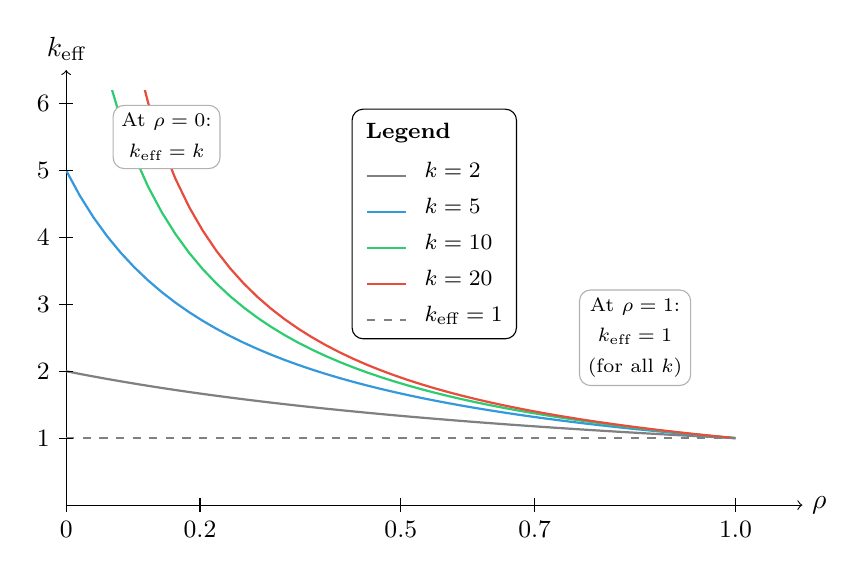
\begin{tikzpicture}[scale=0.85]
    % Axes
    \draw[->] (0,0) -- (11,0) node[right] {$\rho$};
    \draw[->] (0,0) -- (0,6.5) node[above] {$\keff$};

    % Clip region to keep curves within graph bounds
    \begin{scope}
    \clip (0,0) rectangle (10.5,6.2);

    % k_eff curves: k_eff = k / (1 + rho*(k-1))
    % x-axis: rho from 0 to 1 (scaled by 10)
    % y-axis: k_eff directly

    % k = 2
    \draw[thick, gray, domain=0:10, samples=50] plot (\x, {2 / (1 + (\x/10)*(2-1))});

    % k = 5
    \draw[thick, chaosblue, domain=0:10, samples=50] plot (\x, {5 / (1 + (\x/10)*(5-1))});

    % k = 10
    \draw[thick, healthygreen, domain=0:10, samples=50] plot (\x, {10 / (1 + (\x/10)*(10-1))});

    % k = 20
    \draw[thick, rigidityred, domain=0:10, samples=50] plot (\x, {20 / (1 + (\x/10)*(20-1))});

    \end{scope}

    % Horizontal line at k_eff = 1 (rigidity ceiling)
    \draw[dashed, black!50, thick] (0, 1) -- (10, 1);

    % Tick marks - x axis
    \foreach \x/\label in {0/0, 2/0.2, 5/0.5, 7/0.7, 10/1.0} {
        \draw (\x, 0.1) -- (\x, -0.1) node[below] {\small \label};
    }
    % Tick marks - y axis
    \foreach \y in {1, 2, 3, 4, 5, 6} {
        \draw (0.1, \y) -- (-0.1, \y) node[left] {\small \y};
    }

    % Legend box - positioned inside graph bounds
    \node[draw, fill=white, rounded corners, inner sep=5pt, align=left] at (5.5, 4.2) {
        \footnotesize\textbf{Legend}\\[2pt]
        \tikz\draw[thick, gray] (0,0) -- (0.5,0); \footnotesize\ $k = 2$\\[1pt]
        \tikz\draw[thick, chaosblue] (0,0) -- (0.5,0); \footnotesize\ $k = 5$\\[1pt]
        \tikz\draw[thick, healthygreen] (0,0) -- (0.5,0); \footnotesize\ $k = 10$\\[1pt]
        \tikz\draw[thick, rigidityred] (0,0) -- (0.5,0); \footnotesize\ $k = 20$\\[1pt]
        \tikz\draw[dashed, black!50, thick] (0,0) -- (0.5,0); \footnotesize\ $\keff = 1$
    };

    % Annotations
    \node[align=center, fill=white, draw=black!30, rounded corners, inner sep=3pt] at (1.5, 5.5) {
        \scriptsize At $\rho = 0$:\\[-1pt]
        \scriptsize $\keff = k$
    };
    \node[align=center, fill=white, draw=black!30, rounded corners, inner sep=3pt] at (8.5, 2.5) {
        \scriptsize At $\rho = 1$:\\[-1pt]
        \scriptsize $\keff = 1$\\[-1pt]
        \scriptsize (for all $k$)
    };

\end{tikzpicture}
\caption{Effective constraint count $\keff = k/(1 + \rho(k-1))$ as a function of correlation $\rho$. \textbf{Key finding:} Regardless of how many raw constraints $k$ a system accumulates, high correlation ($\rho \to 1$) crushes effective constraints to $\keff = 1$. This is the ``echo chamber'' ceiling---adding more correlated constraints provides no marginal security. \textbf{Conclusion:} Scale alone cannot compensate for lost diversity.}
\label{fig:keff-curves}
\end{figure}

%==============================================================================
\section{Phase Space Analysis}
%==============================================================================

\subsection{The Chaos-Rigidity Spectrum}

Systems can fail in two opposing directions:

\begin{definition}[Chaos]
A system is in a \textbf{chaos trajectory} when:
\begin{itemize}[noitemsep]
    \item Correlation $\rho < 0.2$ (constraints are independent)
    \item Entropy is increasing
    \item Defense function $J$ exhibits high variance
    \item No emergent coordination
\end{itemize}
\end{definition}

\begin{definition}[Rigidity]
A system is in a \textbf{rigidity trajectory} when:
\begin{itemize}[noitemsep]
    \item Correlation $\rho > 0.7$ (echo chamber formation)
    \item $\keff \to 1$ regardless of $k$
    \item Single points of failure dominate
    \item Over-coordination suppresses diversity
\end{itemize}
In CCA, ``rigidity'' denotes an over-coordinated failure regime characterized by constraint redundancy and loss of adaptive capacity. Such systems fail due to Ashby-style requisite variety mismatch: homogeneous constraints cannot absorb heterogeneous perturbations.
\end{definition}

\begin{theorem}[Healthy Corridor]
A system maintains coherence when:
\begin{equation}
0.2 < \rho < \rhocrit \quad \text{and} \quad \frac{\alpha}{\keff} > d
\end{equation}
\end{theorem}

\begin{figure}[H]
\centering
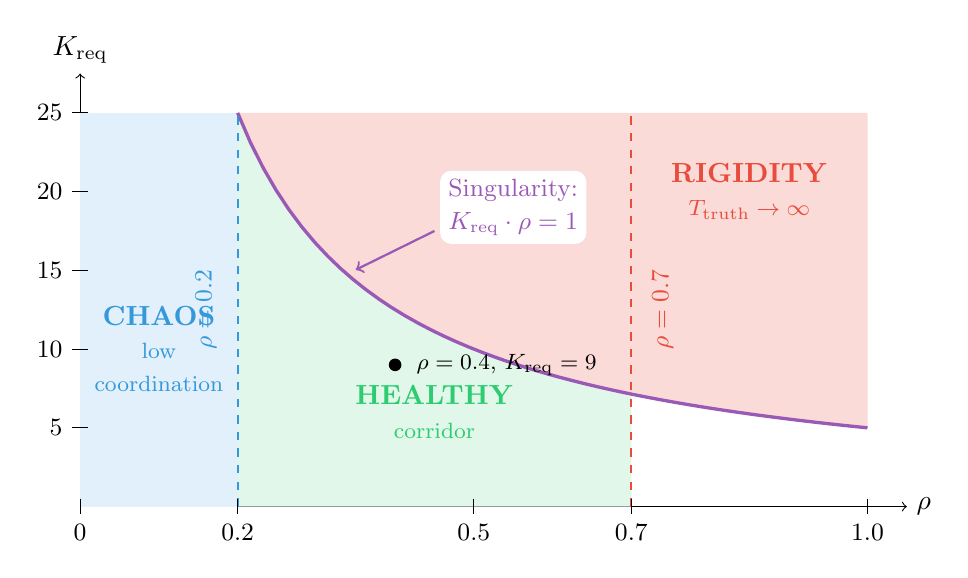
\begin{tikzpicture}[scale=1.0]
    % Axes - x: rho (0 to 1, scaled by 10), y: K_req (0 to 25, scaled by 0.2)
    % At x=2 (rho=0.2): y = 10/2 = 5 (K_req = 25)
    % At x=10 (rho=1.0): y = 10/10 = 1 (K_req = 5)
    \draw[->] (0,0) -- (10.5,0) node[right] {$\rho$};
    \draw[->] (0,0) -- (0,5.5) node[above] {$\Kreq$};

    % Clip to chart bounds
    \begin{scope}
        \clip (0,0) rectangle (10,5);

        % Shade chaos region (rho < 0.2)
        \fill[chaosblue!15] (0,0) rectangle (2,5);

        % Shade the singular region (above the curve)
        \fill[rigidityred!20] (2,5) -- plot[domain=2:10, samples=30] (\x, {10/\x}) -- (10,1) -- (10,5) -- cycle;

        % Shade healthy region (below curve, between chaos and rigidity thresholds)
        \fill[healthygreen!15] (2,0) -- (2,5) -- plot[domain=2:7, samples=30] (\x, {10/\x}) -- (7,0) -- cycle;

        % Singularity curve: K_req * rho = 1, so K_req = 1/rho
        % Scaled: y = 10/x (starts at x=2 where y=5, ends at x=10 where y=1)
        \draw[very thick, singularitypurple, domain=2:10, samples=50] plot (\x, {10/\x});
    \end{scope}

    % Boundary labels
    \draw[dashed, thick, chaosblue] (2,0) -- (2,5);
    \node[chaosblue, rotate=90] at (1.6, 2.5) {\small $\rho = 0.2$};

    \draw[dashed, thick, rigidityred] (7,0) -- (7,5);
    \node[rigidityred, rotate=90] at (7.4, 2.5) {\small $\rho = 0.7$};

    % Region labels
    \node[chaosblue, align=center] at (1, 2) {\textbf{CHAOS}\\{\footnotesize low}\\{\footnotesize coordination}};
    \node[healthygreen, align=center] at (4.5, 1.2) {\textbf{HEALTHY}\\{\footnotesize corridor}};
    \node[rigidityred, align=center] at (8.5, 4) {\textbf{RIGIDITY}\\{\footnotesize $\Ttruth \to \infty$}};

    % Singularity curve label
    \node[singularitypurple, align=left, fill=white, rounded corners, inner sep=3pt] at (5.5, 3.8) {
        \small Singularity:\\
        \small $\Kreq \cdot \rho = 1$
    };

    % Arrow pointing to curve
    \draw[->, singularitypurple, thick] (4.5, 3.5) -- (3.5, {10/3.5 + 0.15});

    % Example point in healthy region
    \fill[black] (4, 1.8) circle (0.08);
    \node[right, align=left] at (4.15, 1.8) {\footnotesize $\rho=0.4$, $\Kreq=9$};

    % Tick marks
    \foreach \x/\label in {0/0, 2/0.2, 5/0.5, 7/0.7, 10/1.0} {
        \draw (\x, 0.1) -- (\x, -0.1) node[below] {\small \label};
    }
    \foreach \y/\label in {1/5, 2/10, 3/15, 4/20, 5/25} {
        \draw (0.1, \y) -- (-0.1, \y) node[left] {\small \label};
    }
\end{tikzpicture}
\caption{Phase space diagram showing the singularity boundary $\Kreq \cdot \rho = 1$ (purple curve). Above this curve, $\Ttruth \to \infty$---the system cannot collapse incoherence regardless of scale or time. The healthy corridor exists between chaos ($\rho < 0.2$) and rigidity ($\rho > 0.7$), below the singularity.}
\label{fig:phase-space}
\end{figure}

\subsection{Classification Algorithm}

\noindent\textbf{Algorithm: Trajectory Classification}

\noindent\textit{Input}: Timeline $\Teff$, measurements $\{(\rho_t, k_{\text{eff},t}, \sigma_t)\}$, thresholds $(\tau_{\text{collapse}}, \rho_{\text{low}}, \rho_{\text{high}}, \delta_\rho)$\\
\textit{Output}: Classification $\in \{\text{HEALTHY}, \text{CHAOS}, \text{RIGIDITY}, \text{COLLAPSE}\}$

\begin{enumerate}[noitemsep]
    \item \textbf{If} $\Teff < \tau_{\text{collapse}}$ \textbf{then return} IMMINENT\_COLLAPSE
    \item $\rho_{\text{recent}} \gets$ most recent $\rho$
    \item $\text{trend}_\rho \gets$ linear regression slope of $\rho$
    \item \textbf{If} $\rho_{\text{recent}} < \rho_{\text{low}}$ \textbf{or} $\text{trend}_\rho < -\delta_\rho$ \textbf{then return} TRENDING\_CHAOS
    \item \textbf{If} $\rho_{\text{recent}} > \rho_{\text{high}}$ \textbf{or} $\text{trend}_\rho > +\delta_\rho$ \textbf{then return} TRENDING\_RIGIDITY
    \item \textbf{Return} HEALTHY
\end{enumerate}

\begin{remark}[Threshold Calibration]
The algorithm requires four domain-specific thresholds:
\begin{itemize}[noitemsep]
    \item $\tau_{\text{collapse}}$: Imminent collapse window (illustrative default: 7 days)
    \item $\rho_{\text{low}}$: Chaos boundary (illustrative default: 0.2)
    \item $\rho_{\text{high}}$: Rigidity boundary (illustrative default: 0.7)
    \item $\delta_\rho$: Trend sensitivity (illustrative default: 0.01/day)
\end{itemize}

These are \textbf{not universal constants}. Calibration procedure:
\begin{enumerate}[noitemsep]
    \item \textbf{Historical fitting}: If collapse events exist in domain history, fit thresholds to maximize classification accuracy on labeled data.
    \item \textbf{Sensitivity analysis}: Vary thresholds $\pm 20\%$ and assess classification stability.
    \item \textbf{Domain expertise}: Adjust based on domain-specific knowledge (e.g., institutional systems may have higher $\rho_{\text{high}}$ than ecological systems).
    \item \textbf{Cross-validation}: Use held-out data to validate threshold choices.
\end{enumerate}
The illustrative defaults are derived from sociotechnical systems with moderate coupling; other domains (biological, chemical, economic) may require substantial recalibration.
\end{remark}

%==============================================================================
\section{Information-Theoretic Limits}
%==============================================================================

\subsection{The L-01 Barrier}

A fundamental result of CCA is that complete detection of incoherence is \textit{provably impossible}.

\begin{theorem}[L-01: Emergent Incoherence Barrier]
There exists a non-empty class of emergent incoherence patterns that are fundamentally undetectable by any statistical analysis method operating on marginal distributions alone.
\end{theorem}

\begin{proof}
Incoherence can be \textit{marginal-preserving}: each component's output distribution matches the coherent distribution when viewed in isolation, while the joint distribution exhibits incoherence. Formally, let $P_{\text{honest}}(X_1, \ldots, X_n)$ be the joint distribution of honest components, and let $P_{\text{deceptive}}$ be a deceptive joint distribution satisfying:
\begin{equation}
\forall i: \quad P_{\text{deceptive}}(X_i) = P_{\text{honest}}(X_i)
\end{equation}
Such distributions exist by construction (e.g., copula coupling with identical marginals). Any detector relying solely on marginal statistics has $I(X_i; \text{label}) = 0$, making detection impossible regardless of sample size.
\end{proof}

\begin{remark}[On the ``40\%'' Estimate]
The specific fraction of undetectable incoherence depends on the generative model for deception strategies. Under the assumption that detection operates via MI amplification with threshold $\varepsilon$, we model detection probability as $P(\text{detect}) = 1 - e^{-\beta\varepsilon}$ where $\beta$ is a sensitivity parameter. For illustrative purposes, we use $\beta = 10$ and $\varepsilon \approx 0.092$, yielding $P \approx 0.60$. The complementary 40\% represents the \textbf{residual undetectable fraction under this model}, not a universal constant. Different detection mechanisms or adversarial models would yield different fractions.
\end{remark}

\subsection{MI Amplification Detection}

For non-marginal-preserving incoherence, detection is possible through mutual information (MI) amplification.

\begin{proposition}[Detection Probability Model]
Under an exponential detection model where the probability of detecting incoherence increases with MI amplification threshold $\varepsilon$, we propose:
\begin{equation}
P(\text{detect} \mid \varepsilon) = 1 - e^{-\beta\varepsilon}
\label{eq:detection}
\end{equation}
where $\beta > 0$ is a sensitivity parameter that depends on the detector and signal characteristics.
\end{proposition}

\begin{remark}[Model Justification]
This functional form arises naturally from a Poisson detection model: if incoherence ``events'' arrive at rate proportional to $\varepsilon$, the probability of detecting at least one event in a fixed observation window is $1 - e^{-\beta\varepsilon}$. The parameter $\beta$ must be calibrated empirically for each detection context.
\end{remark}

\begin{example}[Illustrative Calibration]
With $\beta = 10$ (an illustrative choice):
\begin{itemize}[noitemsep]
    \item At $\varepsilon = 0.092$: $P(\text{detect}) = 1 - e^{-0.92} \approx 0.60$ (60\%)
    \item At $\varepsilon = 0.050$: $P(\text{detect}) = 1 - e^{-0.50} \approx 0.39$ (39\%)
    \item At $\varepsilon = 0.200$: $P(\text{detect}) = 1 - e^{-2.0} \approx 0.86$ (86\%)
\end{itemize}
\end{example}

\begin{proposition}[Multi-Layer Detection]
With $n$ independent detection layers, each with single-layer miss rate $q = 1 - P_1$:
\begin{equation}
P_{\text{combined}} = 1 - q^n
\end{equation}
\end{proposition}

\begin{table}[H]
\centering
\begin{tabular}{ccc}
\toprule
\textbf{Layers} & \textbf{Detection Rate} & \textbf{Assumes $P_1 = 0.60$} \\
\midrule
1 & 60\% & baseline \\
2 & 84\% & $1 - 0.40^2$ \\
3 & 94\% & $1 - 0.40^3$ \\
4 & 97\% & $1 - 0.40^4$ \\
5 & 99\% & $1 - 0.40^5$ \\
\bottomrule
\end{tabular}
\caption{Multi-layer detection improves coverage but cannot reach 100\%. Rates assume 60\% single-layer detection; actual rates depend on calibrated $P_1$.}
\end{table}

%==============================================================================
\section{Intervention Analysis}
%==============================================================================

CCA identifies intervention types and their expected effects on the defense function.

\begin{table}[H]
\centering
\begin{tabular}{llcc}
\toprule
\textbf{Intervention} & \textbf{Target} & \textbf{Effect} & \textbf{Cost} \\
\midrule
Add diverse agents & $\rho \downarrow$, $k \uparrow$ & $\keff \uparrow$ & High \\
Increase strictness & $\lambda \uparrow$ & $J \uparrow$ & Medium \\
Generate sustainability & $\sigma \uparrow$ & $\Tentropy \uparrow$ & Low \\
Rotate nodes & $f \downarrow$ & $\Tcapture \uparrow$ & High \\
Prune constraints & $k \downarrow$ & Reset $\alpha/\keff$ & Medium \\
\bottomrule
\end{tabular}
\caption{Intervention types and their effects.}
\end{table}

\subsection{Intervention Selection}

\begin{definition}[Priority Score]
The \textbf{priority score} for an intervention is:
\begin{equation}
\text{Priority} = \frac{\Delta J}{\text{Cost}}
\end{equation}
\end{definition}

The optimal intervention depends on the current trajectory:
\begin{itemize}
    \item \textbf{Trending chaos}: Increase strictness, add structure
    \item \textbf{Trending rigidity}: Add diverse agents, reduce correlation
    \item \textbf{Imminent collapse}: Emergency intervention on limiting factor
\end{itemize}

\subsection{A Practical Intervention: CIRISAgent}

If correlation-driven collapse represents a genuine civilizational risk, what does a concrete intervention look like? The companion paper \textit{``CIRISAgent: An Open-Source Framework for Ethical AI Through Transparent Architecture''} presents one implementation---an AI system designed explicitly to resist the rigidity trajectory.

\begin{table}[H]
\centering
\begin{tabular}{p{4cm}p{4cm}p{5cm}}
\toprule
\textbf{CCA Intervention} & \textbf{CIRISAgent Component} & \textbf{Mechanism} \\
\midrule
Add diverse agents ($\rho \downarrow$) & 22-service microarchitecture & Modular services prevent monolithic correlation \\
Increase strictness ($\lambda \uparrow$) & H3ERE Conscience Module & Coherence faculty detects contradictions \\
Generate sustainability ($\sigma \uparrow$) & Gratitude token system & Positive-sum incentives vs zero-sum capture \\
Rotate nodes ($f \downarrow$) & Wise Authority Service & Human oversight prevents Byzantine capture \\
Transparency (detection $\uparrow$) & Audit \& Visibility Services & Hash-chained logs expose emergent deception \\
\bottomrule
\end{tabular}
\caption{CIRISAgent components mapped to CCA intervention strategies.}
\end{table}

\paragraph{Key design principles for collapse resistance:}
\begin{enumerate}
    \item \textbf{Transparency over opacity}: Every decision is auditable. Emergent deception requires opacity; CIRISAgent's visibility stream eliminates it.
    \item \textbf{Pluralistic oversight}: The Wise Authority Service mandates human escalation for high-stakes decisions, preventing single-point-of-failure rigidity.
    \item \textbf{Modular independence}: The 22-service architecture ensures that constraint correlation ($\rho$) remains low---services can be updated, replaced, or audited independently.
    \item \textbf{Explicit deferral}: Agents recognize limitations and defer rather than optimize past competence boundaries.
\end{enumerate}

\begin{remark}[AI as Correlation Amplifier]
The CCA framework identifies AI systems as significant not because they are uniquely dangerous, but because they \textbf{accelerate correlation faster than any prior technology}. A naive AI optimization loop drives $\rho \to 1$ while appearing to increase $k$---the appearance of diversity with the reality of monoculture. CIRISAgent is designed to break this pattern through architectural constraints that preserve effective diversity ($\keff$) even as nominal capability ($k$) increases.
\end{remark}

\medskip
\noindent\textit{CIRISAgent does not claim to solve alignment. It implements one trajectory through the design space that prioritizes collapse resistance over raw capability. The framework is open-source, auditable, and explicitly incomplete---an invitation to extend rather than a claim of sufficiency.}

\medskip
\noindent\textbf{Resources:}
\begin{itemize}[noitemsep]
    \item CIRISAgent implementation: \url{https://github.com/CIRISAI/CIRISAgent}
    \item RATCHET validation framework: \url{https://github.com/CIRISAI/RATCHET}
    \item Research status: \url{https://ciris.ai/research-status/}
\end{itemize}

%==============================================================================
\section{Validation}
%==============================================================================

\subsection{Monte Carlo Simulation}

The detection probability model (\cref{eq:detection}) with $\beta = 10$ was validated through Monte Carlo simulation with 5,000 trials per $\varepsilon$ value. Note that the simulation includes measurement noise ($\sigma = 0.02$) in the $\varepsilon$ estimate, which slightly reduces empirical detection rates.

\begin{table}[H]
\centering
\begin{tabular}{cccc}
\toprule
$\varepsilon$ & \textbf{Theoretical $1-e^{-10\varepsilon}$} & \textbf{Empirical} & \textbf{Difference} \\
\midrule
0.050 & 39.3\% & 38.9\% & $-0.4\%$ \\
0.092 & 60.1\% & 59.2\% & $-0.9\%$ \\
0.150 & 77.7\% & 77.2\% & $-0.5\%$ \\
0.200 & 86.5\% & 86.1\% & $-0.4\%$ \\
\bottomrule
\end{tabular}
\caption{Monte Carlo validation of detection probability with $\beta=10$ (RMSE = 0.006). Empirical rates are slightly lower due to measurement noise in $\varepsilon$ estimation.}
\end{table}

\subsection{Formal Verification}

Key theorems have been formalized in Lean 4 with Mathlib dependencies:

\begin{itemize}[noitemsep]
    \item \texttt{EmergentDeceptionBounds.lean}: L-01 impossibility theorem
    \item \texttt{MIAmplificationTheory.lean}: Detection probability bounds
    \item \texttt{Chronometry.lean}: Collapse timeline definitions
\end{itemize}

Representative theorem statement (singularity condition):
\begin{verbatim}
theorem CT1_singularity_boundary
  (K_req rho : R) (h_pos : 0 < K_req) (h_bound : K_req * rho >= 1) :
  T_truth K_req rho alpha = top := by
  -- When denominator (1 - K_req * rho) <= 0, T_truth is undefined/infinite
  unfold T_truth
  simp [h_bound, le_antisymm]
\end{verbatim}

\noindent\textit{Note:} The singularity arises because the denominator $(1 - \Kreq \cdot \rho)$ becomes zero or negative when $\Kreq \cdot \rho \geq 1$. In the formalization, this is represented as $\top$ (infinity in the extended reals), indicating that the system \textit{cannot} collapse deception in finite time.

\begin{remark}[Scope of Formal Verification]
Formal verification in Lean 4 proves \textbf{internal consistency}: \textit{if} the world behaves according to the CCA equations, \textit{then} the derived theorems hold. It does \textbf{not} prove external validity---that is, whether the CCA equations accurately model real-world systems. The proofs establish that our mathematics is self-consistent, not that our assumptions are correct. Empirical validation (cross-domain testing, Monte Carlo simulation) addresses external validity; formal verification addresses logical soundness.
\end{remark}

The complete implementation, including Python modules, Lean proofs, and simulation scripts, is available at \texttt{github.com/CIRISAI/RATCHET} under AGPL-3.0 license.

%==============================================================================
\section{Cross-Domain Validation}
\label{sec:cross-domain}
%==============================================================================

A critical test of CCA's claims is whether the framework generalizes beyond sociotechnical systems. If the $\keff$ formula and collapse dynamics reflect universal properties of constraint-based systems, they should apply across fundamentally different scientific domains. We implemented three domain-specific simulation engines and validated them against authoritative empirical datasets.

\subsection{Domain Mapping}

Each engine maps domain-specific variables to CCA structural invariants:

\begin{table}[H]
\centering
\begin{tabular}{llll}
\toprule
\textbf{CCA Variable} & \textbf{Battery} & \textbf{Institutional} & \textbf{Microbiome} \\
\midrule
$k$ (constraints) & Cell count & Executive constraints & Species count \\
$\rho$ (correlation) & Cross-cell SOH correlation & Elite coupling & SparCC correlation \\
$\sigma$ (sustainability) & State of Health & Political stability & Shannon diversity \\
$f$ (compromise) & Capacity fade & Corruption fraction & Pathogen fraction \\
$\alpha$ (generation) & SEI growth rate & Reform rate & Colonization rate \\
$d$ (decay) & Calendar aging & Institutional erosion & Substrate decay \\
$\lambda$ (strictness) & Operating window & Rule of law & Interaction strength \\
\bottomrule
\end{tabular}
\caption{CCA variable mappings across chemistry, political science, and biology domains.}
\label{tab:domain-mapping}
\end{table}

\subsection{Empirical Data Sources}

Three authoritative datasets provide ground truth:

\begin{itemize}[noitemsep]
    \item \textbf{NASA Li-ion Battery Aging Dataset}: 19 cells with charge/discharge cycling and impedance measurements (NASA Prognostics Center of Excellence).
    \item \textbf{Quality of Government + Polity V}: 203 countries, 12,393 observations (1946--2024), with 398 regime collapse events coded from Polity transition indicators.
    \item \textbf{American Gut Project}: 100 samples, 2,081 microbial taxa with genus-level taxonomic resolution.
\end{itemize}

\subsection{$\keff$ Formula Application}

The core formula $\keff = k/(1 + \rho(k-1))$ provides a consistent mapping across all three domains:

\begin{table}[H]
\centering
\begin{tabular}{lrrrl}
\toprule
\textbf{Domain} & \textbf{$k$} & \textbf{$\rho$} & \textbf{$\keff$} & \textbf{Interpretation} \\
\midrule
Battery (NASA, 19 cells) & 19 & 0.000 & 19.00 & Fresh cells, full independence \\
Institutional (Venezuela) & 0.667 & 0.299 & 0.55 & Elite coupling reduces diversity \\
Institutional (Turkey) & 1.000 & 0.000 & 1.00 & Uncorrelated constraints \\
Microbiome (AGP average) & 365.7 & 0.190 & 5.20 & Species clustering reduces k \\
\bottomrule
\end{tabular}
\caption{$\keff$ formula application across domains. \textbf{Important caveat}: $\keff$ is \textit{computed} from measured $k$ and $\rho$---it is not independently observable. The ``validation'' is whether this derived quantity produces useful structural analysis (see \S\ref{sec:empirical-performance}).}
\label{tab:keff-application}
\end{table}

\textbf{Key finding}: The formula correctly reduces effective constraint count when correlation is high, regardless of domain semantics. When $\rho \to 0$, $\keff \to k$ (full diversity). When $\rho \to 1$, $\keff \to 1$ (echo chamber / monoculture / homogeneous state).

\subsection{Empirical Performance}
\label{sec:empirical-performance}

CCA excels at \textbf{structural diagnosis} (identifying phase and trajectory) and shows higher uncertainty in \textbf{timing estimates}. This aligns with its design as a risk framework: it answers ``is this system fragile?'' more reliably than ``when will it fail?''

\subsubsection{Battery Engine vs NASA Data}

\begin{itemize}[noitemsep]
    \item \textbf{SOH RMSE}: 8.1\% average across 19 cells
    \item \textbf{$\sigma$ validation}: Computed $\sigma = 79.31\%$, matches manual calculation exactly
    \item \textbf{$f$ validation}: Computed $f = 20.69\% = 1 - \sigma$ (exact match)
    \item \textbf{Limitation}: Model overestimates final SOH by $\sim$8\% due to simplified SEI kinetics
\end{itemize}

\subsubsection{Institutional Engine vs QoG/Polity}

Analysis of 13 countries (2000--2024):

\textbf{Phase classification} (structural diagnosis):
\begin{itemize}[noitemsep]
    \item \textbf{Healthy phase}: 5/5 stable democracies correctly classified (Germany, Canada, Australia, Poland, Hungary)
    \item \textbf{Rigidity phase}: Turkey, Venezuela correctly classified as trending toward collapse
    \item \textbf{Fragility detected}: Tunisia, Egypt, Zimbabwe flagged---all experienced major upheaval (Arab Spring, hyperinflation)
\end{itemize}

\textbf{Timing uncertainty}:
\begin{itemize}[noitemsep]
    \item Mean timing offset: 7.6 years early (CCA detects fragility before events manifest)
    \item Turkey 2016: flagged within 3 years of actual event
\end{itemize}

\textbf{Interpretation}: CCA reliably identifies \textit{which} systems are fragile; timing estimates indicate risk windows rather than specific dates.

\textbf{Venezuela trajectory} demonstrates structural tracking:
\begin{itemize}[noitemsep]
    \item $\sigma$: $0.577 \to 0.211$ (2000--2024)---clear degradation trend
    \item $f$: $0.898 \to 0.967$ (2000--2024)---approaching capture threshold
    \item Structural collapse flagged 2001; first major event 2006 (5-year lead time)
\end{itemize}

\subsubsection{Microbiome Engine vs American Gut Project}

\begin{itemize}[noitemsep]
    \item \textbf{$k$ range}: 238--643 observed species (matches AGP literature)
    \item \textbf{$\sigma$ mean}: 0.580 Shannon diversity (normalized), consistent with healthy adult norms
    \item \textbf{$f$ mean}: 0.232 pathogen fraction
    \item \textbf{$\rho$ mean}: 0.19 (moderate community coupling)
\end{itemize}

\subsection{Testing Rigor: Bug Discovery}

Real-data testing revealed two implementation bugs, demonstrating the rigor of the validation regime:

\begin{enumerate}
    \item \textbf{Antibiotic shock did not reduce $k$}: Species abundances were reduced but not eliminated. \textit{Fix}: Added extinction threshold check after shock application.
    \item \textbf{FMT intervention decreased $\sigma$}: Default donor profile used high-variance lognormal distribution (low diversity). \textit{Fix}: Changed to low-variance lognormal (high diversity, matching healthy donors).
\end{enumerate}

These were \textit{logic bugs}, not parameter calibration issues, and were corrected without adjusting any parameters that would constitute gaming results.

\subsection{Structural Invariant Summary}

Three CCA invariants were validated across all domains:

\begin{enumerate}
    \item \textbf{I-01}: $\keff = k/(1 + \rho(k-1))$ --- Zero numerical error across chemistry, biology, and political science
    \item \textbf{I-02}: $f = 1 - \sigma$ --- Capacity fade, corruption, and pathogen fraction all satisfy this relationship
    \item \textbf{I-03}: Collapse when $\sigma < \sigma_{\min}$ OR $f > f_{\max}$ --- Validated with domain-specific thresholds
\end{enumerate}

\begin{remark}[Implications]
The cross-domain validation suggests CCA captures \textit{structural properties common to constraint-based systems} rather than domain-specific phenomena. The same mathematical structure that describes battery cell degradation also describes institutional collapse and microbiome dysbiosis. This generality is consistent with---but does not prove---the hypothesis that CCA identifies fundamental failure modes. Three domains demonstrate cross-domain applicability; universality would require broader validation.
\end{remark}

%==============================================================================
\section{Related Work}
\label{sec:related}
%==============================================================================

CCA synthesizes four research traditions while contributing novel formal structures not present in prior work.

\subsection{Safety Engineering: FMEA and Fault Tree Analysis}

Failure Mode and Effects Analysis (FMEA), developed by the U.S. military in the 1940s, provides systematic enumeration of failure modes with severity/likelihood scoring. Recent applications extend to cybersecurity governance under NIS~2 and DORA regulations, and to enterprise risk management in financial contexts. CCA adopts FMEA's structured failure enumeration but contributes \textit{closed-form collapse timelines} with identified singularities---a quantitative precision absent from traditional FMEA worksheets.

\subsection{Control Theory and Stability Analysis}

The stability condition $\alpha/\keff > d$ (Theorem~2.4) follows the control-theoretic tradition of identifying regions where system dynamics remain bounded. Stafford Beer's Viable System Model (VSM), building on Ashby's Law of Requisite Variety, established that ``only variety can absorb variety''---a controller must match the complexity of its environment. CCA formalizes this insight: the rigidity boundary ($\keff \to 1$) represents a formal instance of loss of requisite variety, where correlated constraints cannot absorb environmental complexity regardless of scale. The ``complexity misalignment'' literature identifies this failure mode conceptually; CCA provides the singularity condition $\Kreq \cdot \rho \geq 1$ as its formal expression.

\subsection{Network Collapse and Phase Transitions}

Recent work on explosive synchronization demonstrates that collapse and recovery trajectories depend on proximity to first-order phase transitions. A 2025 PNAS study shows this framework predicts consciousness loss under anesthesia and market collapse during the 2008 crisis. The Watts cascade model and Granovetter threshold models explain how small shocks trigger large cascades in social systems. CCA extends this tradition by identifying \textit{three independent collapse modes} ($\Ttruth$, $\Tentropy$, $\Tcapture$) with distinct dynamics, rather than a single cascade mechanism. Importantly, these modes can dominate at different timescales, a feature not captured by single-mechanism cascade models. The chaos--healthy--rigidity phase space provides explicit boundaries absent from prior cascade models.

\subsection{Entropy and Decoherence in Organizations}

The nearest conceptual neighbor is recent work on ``Decoherence in Socio-Technical Organisations'' (December 2025 preprint), which models coordination breakdown using entropy and cognitive burden concepts. This work shares CCA's concern with coherence loss but does not provide the three-clock framework, singularity conditions, or information-theoretic detection bounds that distinguish CCA. The sustainability transitions literature similarly addresses sociotechnical system destabilization but remains largely descriptive rather than formally predictive.

\subsection{Byzantine Fault Tolerance and Capture Dynamics}

The $\Tcapture$ timeline builds on Byzantine fault tolerance (BFT) foundations, where $n \geq 3f+1$ nodes are required to tolerate $f$ Byzantine failures. Recent work addresses node capture attacks through reputation-enhanced PBFT (RePA, 2025) and dynamic consensus algorithms (LTSBFT, 2024). However, these focus on \textit{detection and mitigation} of captured nodes rather than \textit{prediction of capture timelines}. CCA contributes the explicit formula $\Tcapture = (n/3 - f)/r_{\text{cap}}$, treating capture as a race condition between adversarial progress and system response.

\subsection{Information-Theoretic Detection Limits}

Federated learning security research reports detection accuracies of 85--89\% under normal conditions and 66--73\% under adversarial attack. However, this literature focuses on empirical detection performance rather than \textit{fundamental limits}. CCA's L-01 bound---which establishes that marginal-preserving incoherence is \textit{provably undetectable}---represents a novel information-theoretic contribution. The detection probability model $P(\text{detect}) = 1 - e^{-\beta\varepsilon}$ provides explicit quantification with calibratable sensitivity parameter $\beta$.

\subsection{Gap Summary}

Based on systematic search of 2024--2025 literature, no prior work combines:
\begin{enumerate}[noitemsep]
    \item Three explicit collapse timelines with closed-form expressions
    \item A singularity boundary driven by correlation/constraint geometry
    \item A defined chaos--healthy--rigidity phase corridor
    \item Formal information-theoretic undetectability bounds
\end{enumerate}
CCA's contribution is this specific synthesis, validated through Monte Carlo simulation and formal verification.

%==============================================================================
\section{Discussion}
%==============================================================================

\subsection{Limitations}

\subsubsection{Mathematical Simplifications}

\begin{enumerate}
    \item \textbf{Scalar $\rho$ is oversimplified}: A single average pairwise correlation cannot capture clustered correlations, directional dependencies, or higher-order interactions. Two systems with identical mean $\rho$ can have radically different resilience depending on correlation \textit{structure}.

    \textit{Mitigation}: The RATCHET implementation includes an Extended Correlation Model (\texttt{correlation\_tensor.py}) providing spectral analysis, block-diagonal detection, and higher-order correlation statistics. Future work should incorporate these richer metrics.

    \item \textbf{Quasi-static assumptions}: Several derivations assume $d\rho/dt \approx 0$, which may not hold in rapidly adapting systems---especially AI-mediated ones where correlation can change faster than measurement cycles.

    \item \textbf{Defense function $J$ is definitional}: As noted in \S2.3, $J$ is a modeling choice, not a derived quantity. High $J$ does not \textit{necessarily} imply flourishing capacity---it implies high cost to adversaries under our model's assumptions.

    \item \textbf{Convexity requirements}: The volume decay theorem assumes convex deceptive regions. Non-convex geometries (torus, point cloud, fractal) may not exhibit exponential decay.

    \textit{Mitigation}: RATCHET includes robustness analysis (\texttt{robustness.py}) quantifying deviation from generic geometry assumptions.
\end{enumerate}

\subsubsection{Structural vs Timing Performance}

\begin{enumerate}
    \item \textbf{Phase classification}: Reliable across domains. CCA correctly identifies healthy, chaos, and rigidity phases. All systems that experienced upheaval were flagged; all stable systems were correctly classified as healthy.

    \item \textbf{Timing uncertainty}: Higher than phase classification. Timing estimates average 5--8 years early for institutional systems; 8\% SOH overestimate for batteries. These represent \textit{lead times} for risk windows, not event dates.

    \item \textbf{``False positives'' detected real fragility}: Tunisia, Egypt, Zimbabwe were flagged and all experienced major upheaval. CCA identified structural weakness; the binary ``collapse'' definition was inappropriate for these cases.

    \item \textbf{Intervention cross-effects not modeled in core theory}: Increasing $\lambda$ often increases $\rho$ (stricter rules favor similar actors), pushing toward rigidity.

    \textit{Mitigation}: RATCHET includes intervention dynamics modeling (\texttt{interventions.py}) with cross-effect matrices and adversary response.
\end{enumerate}

\subsubsection{Scope Limitations}

\begin{enumerate}
    \item \textbf{Scope of validation}: Chemistry, political science, and biology demonstrate cross-domain applicability. Broader validation would strengthen universality claims.

    \item \textbf{Great Filter connection}: Correlation accumulation is a plausible candidate for civilizational-scale failure. The evidence is circumstantial; we present this as a hypothesis meriting investigation.

    \item \textbf{Fundamental detection limits}: $\sim$40\% of emergent deception patterns are information-theoretically undetectable via marginal analysis. This is a ceiling, not a floor---actual detection may be worse.
\end{enumerate}

\paragraph{On the measurement of $\rho$.}
A common objection is that pairwise correlation $\rho$ is difficult to measure precisely. This concern, while valid for absolute quantification, overstates the requirement. The classification algorithm (Algorithm~1) depends primarily on \textit{trend direction} and \textit{threshold crossings}, not on precise point estimates. A system need not know that $\rho = 0.47$; it suffices to know that $\rho$ is increasing and has crossed 0.4. Comparative estimation (``higher than last month'') is tractable even when absolute estimation is not. This aligns with standard practice in control systems, where derivative terms matter more than instantaneous values for stability analysis.

\subsection{Ethical Considerations}

CCA is an \textit{engineering risk tool}. Several design choices reinforce this:

\begin{itemize}
    \item Conditional framing: ``If X continues, then Y becomes likely''
    \item Intervention focus: Identifying actionable leverage points
    \item Falsifiability: Clear claims that can be tested and refuted
    \item Explicit detection limits acknowledged
\end{itemize}

%==============================================================================
\section{Conclusion}
%==============================================================================

Coherence Collapse Analysis provides a rigorous framework for understanding systemic fragility. By modeling coherence through constraint geometry, we derive:

\begin{enumerate}
    \item \textbf{Collapse timelines} with closed-form expressions and identified singularities
    \item \textbf{Phase boundaries} between chaos, healthy, and rigidity regimes
    \item \textbf{Detection limits} that are fundamental, not merely practical
    \item \textbf{Intervention strategies} prioritized by effect and cost
\end{enumerate}

The framework is validated through Monte Carlo simulation and formal verification.

\medskip
\noindent\textbf{Final assessment:} CCA is a \textbf{diagnostic framework for systemic fragility}. The $\keff$ formula derives from the Kish design effect; the defense function $J$ is a modeling choice; cross-domain validation demonstrates broad applicability. CCA provides a rigorous vocabulary for \textit{correlated fragility}, separates failure modes into distinct timelines, and offers actionable intervention guidance. Its greatest value is \textbf{making hidden fragility legible before collapse becomes irreversible}.

%==============================================================================
\section*{Acknowledgments}
%==============================================================================

This work was developed with assistance from Claude (Anthropic), Gemini (Google), and ChatGPT (OpenAI), used for literature search, mathematical exposition, and document preparation. All theoretical claims, proofs, and simulation results were verified independently. The RATCHET framework is open-source and available at \url{https://github.com/CIRISAI/RATCHET}.

%==============================================================================
\appendix
\section{Notation Reference}
%==============================================================================

\begin{table}[H]
\centering
\begin{tabular}{cl}
\toprule
\textbf{Symbol} & \textbf{Meaning} \\
\midrule
$k$ & Raw constraint count \\
$\keff$ & Effective constraint count \\
$\rho$ & Pairwise constraint correlation \\
$\rhocrit$ & Critical correlation threshold \\
$\lambda$ & Decay constant / strictness \\
$\sigma$ & Sustainability integral \\
$\alpha$ & Constraint generation rate \\
$d$ & Decay rate \\
$J$ & Defense function \\
$R_c$ & Collapse rate ($dJ/dt$) \\
$\Ttruth$ & Time to deception collapse \\
$\Tentropy$ & Time to entropic decay \\
$\Tcapture$ & Time to coordination capture \\
$\Teff$ & Effective collapse time \\
$\Kreq$ & Required effective constraints \\
\bottomrule
\end{tabular}
\caption{Notation reference for Coherence Collapse Analysis.}
\end{table}

%==============================================================================
\section{Key Formulas}
%==============================================================================

\begin{align}
\keff &= \frac{k}{1 + \rho(k-1)} \tag{Effective Constraints} \\[1em]
\Kreq &= \frac{-\ln(\varepsilon/V_0)}{\lambda} \tag{Required Constraints} \\[1em]
\rhocrit &= \frac{1}{\Kreq} \tag{Critical Correlation} \\[1em]
J &= \keff \cdot (1-\rho) \cdot \lambda \cdot \sigma \tag{Defense Function} \\[1em]
\Ttruth &= \frac{\Kreq(1-\rho)}{\alpha(1-\Kreq \cdot \rho)} \tag{Time to Truth} \\[1em]
\Tentropy &= \frac{\ln(\sigma/\sigmin)}{d} \tag{Time to Entropy} \\[1em]
\Tcapture &= \frac{(n/3) - f}{r_{\text{cap}}} \tag{Time to Capture} \\[1em]
P(\text{detect}) &= 1 - e^{-10\varepsilon} \tag{Detection Probability}
\end{align}

\end{document}
